\documentclass[a4paper,english]{article}
\usepackage{graphicx}
\usepackage{listings}
\usepackage{amsmath}
\usepackage{multirow}

%% Use utf-8 encoding for foreign characters
%%\usepackage[T1]{fontenc}
%%\usepackage[utf8]{inputenc}
%%\usepackage{babel}
%%
%%%% Vector based fonts instead of bitmaps
%%\usepackage{lmodern}
%%
%%%% Useful
%%%\usepackage{fullpage} % Smaller margins
%%\usepackage{enumerate}
%%
%%%% Theorem
%%\usepackage{amsthm}
%%
%%%% More math
%%\usepackage{amsmath}
%%\usepackage{amssymb}
\lstset{
  breaklines=true,
  postbreak=\mbox{{$\hookrightarrow$}\space},
  backgroundcolor = \color{lightgray},
}

%% Document Header
\title{Section1}
\author{Elliott Ashby}
\date{\today}

\begin{document}
    \maketitle
    \section{q1}
    \lstinputlisting[language=Python, firstline=4, lastline=15]{q1.py}
    The above code first defines the integrad, $f(x)$, and then the function trap0, which takes the integrand, and upper and lower bound and the number of strips to use.
    \section{q2}
    Calling the functions in the following way can calculate the value of the integral.
    \lstinputlisting[language=Python, firstline=, lastline=]{q1.py}
    Running this will give an output for the value of:
    \begin{center}
        $\int_0^1{\frac{x^4(1-x)^4}{1+x^2}dx} = 0.0012649570769764054$
    \end{center}
    \section{q3}
    Which was achieved using 7 strips.
    \section{q4}
    \lstinputlisting[language=Python, firstline=, lastline=]{q1.py}
    Which will calculate:
    \begin{center}
            $\int_{-a}^a{e^{-x^2}dx} = 1.7724538509055157$
    \end{center}
    Where a increases by one every iteration. \\
    This produces an output of:
    \begin{center}
         $1.4931691935764426, 1.7639724905315541, 1.7723984788565614, 1.7724537930187396, 1.7724538509008183, 1.7724538509055159, 1.772453850905516, 1.772453850905516, 1.7724538509056167, 1.7724538509055157$
    \end{center}
    \section{q5}
    \begin{center}
        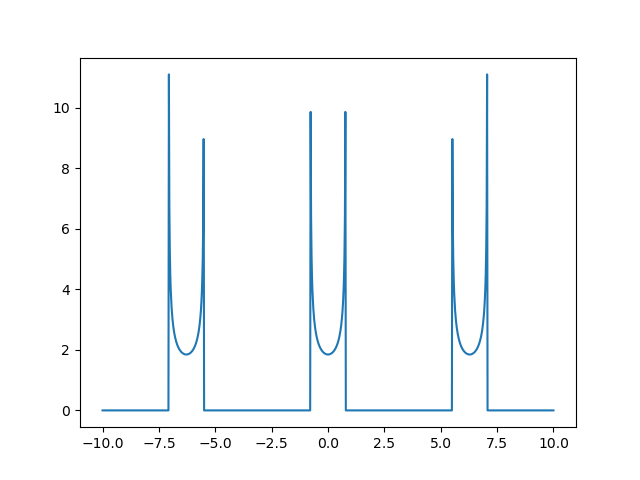
\includegraphics[scale=0.8]{./3_5.png}
    \end{center}
    \begin{center}
        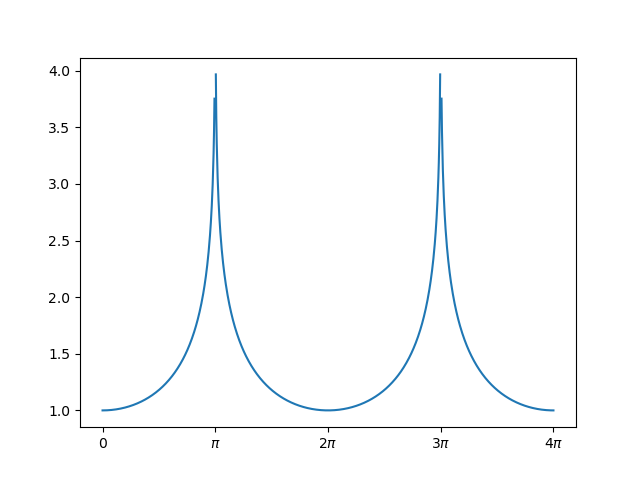
\includegraphics[scale=0.8]{./3_6.png}
    \end{center}
    \section{q6}
    

\end{document}
